%%%%%%%%%%% Aquí va la solución al problema 1.
\newpage
\textbf{\textcolor{MidnightBlue}{2.}}
Demuestra que el algoritmo 2 soluciona el problema del consenso en una gráfica G arbitraria, tolerando
$f < k(G)$ fallas de tipo paro. $k(G)$ denota la conexidad por vértices de G, es decir, el mínimo
número de vértices que se tienen que quitar de $G$ para desconectarla. Entonces, si hay menos de $k(G)$
fallas de los procesos, la gráfica que queda sigue siendo conexa. Tip: Piensa que tanto tarda en fluir la
entrada mínima más pequeña, a pesar de las fallas que puedan ocurrir.\\


\begin{center}
    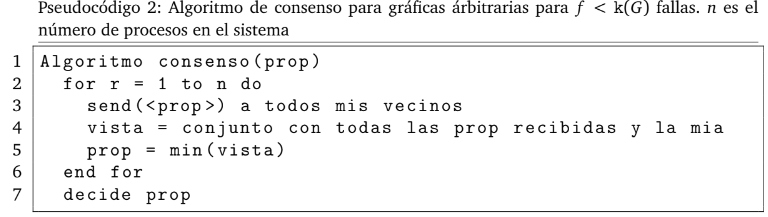
\includegraphics[scale=0.6]{consensoProblema2.png}
    \end{center}
